
\chapter{Introducción}
\label{cha:introduccion}

\section{Sobre el documento} 

El objeto principal de este trabajo es obtener un algoritmo que permita obtener
el diagrama de radiación en campo lejano a partir de las medidas del campo
eléctrico medido en la zona denominada por contra como de campo cercano
radiado por una antena.
\\

Para ello, y dado que la idea principal es poder aplicar lo estudiado en este documento sobre medidas reales, nos hemos ceñido al estándar IEEE Std-149-2021. Este es el estándar vigente a fecha de escritura de este
documento, y define todo lo referente a la toma de medidas de una antena.\\
Con su ayuda estableceremos una serie de reglas y asunciones que conviene detallar desde el principio, por lo que esta sección introductoria servirá a este propósito.
\\

De todo lo definido por el estándar 149-2021 \autocite{IEEEstd} nos interesan dos ideas fundamentales. La primera es que vamos a centrarnos en el estudio de antenas pasivas, lineales y recíprocas. Esto implica que podemos medir sus propiedades independientemente de si durante el estudio la establecemos como transmisor o receptor.
\\

No obstante, es importante recalcar que el propio estándar afirma que gran parte de las prácticas pueden adaptarse al caso de medir sistemas que contengan elementos activos, no lineales o no recíprocos. Así, pese a que este documento ignora este tipo de sistemas, lo descrito en él podría aplicarse a dichos casos particulares.
\\
El segundo punto clave a tener en cuenta es que el estándar, y por extensión este documento, prioriza la obtención del patrón de radiación de la antena bajo estudio. Esto se debe a que es una propiedad fundamental de cualquier antena a partir de la cual podemos obtener características como la directividad, la ganancia o la eficiencia de radiación, y haciendo uso también de otras medidas disponibles en el analizador de redes con el que trabajamos.
\\
\newpage
\section{Sobre la toma de medidas}

La base principal para poder efectuar medidas sobre una antena es disponer de una instalación que cumpla una serie de requisitos muy concretos. Esto se debe a que usualmente las antenas no pueden ser caracterizadas de forma analítica por culpa de sus complejas configuraciones estructurales y sus diferentes métodos de excitación. Incluso con la tecnología actual, pese a haber reducido el número de antenas de difícil medición gracias a métodos de estimaciones como el “Moment Method” o el “Finite-Difference Time-Domain” (siendo este último el método empleado para simular la electromecánica computacionalmente), siguen existiendo varias antenas muy difíciles de medir de forma analítica.\\ 

Este hecho implica que debemos emplear métodos experimentales para validar nuestros resultados teóricos donde preferiblemente situaremos la antena que queremos caracterizar en modo receptor. Además, si la antena que vamos a medir es recíproca, significa que tendrá el mismo comportamiento en modo receptor y transmisor, es decir, su ganancia, eficiencia y patrón de radiación son idénticos independientemente del uso que le demos a la antena. Sabiendo esto, la condición ideal para medir las características de radiación del campo lejano consiste en transmitir ondas planas como radiación incidente sobre la antena que queramos medir. Recordemos que las ondas planas son ondas de amplitud constante y uniforme que presentan frentes de onda planos. En la práctica, esta condición ideal no es alcanzable, pero podemos obtener una aproximación si situamos en el exterior las antenas y las separamos una distancia tal que permita que la onda transmitida se asemeje a una onda plana al llegar a la antena receptora. Sin embargo, este método presenta los siguientes inconvenientes:

\begin{itemize}
    \item A nivel físico, si realizásemos un despliegue real en el exterior sobre el que efectuar medidas, nunca podremos saber si los datos medidos pertenecen al comportamiento de la antena o si por el contrario están contaminados por interferencias u otros fenómenos que puedan contaminar las medidas. En otras palabras, los sistemas de medición externos proporcionan un entorno no controlado.
    \item A nivel material, si queremos aislar las antenas de perturbaciones externas necesitaríamos disponer de una infraestructura que fuese capaz de albergar toda la distancia necesaria para recrear una situación de despliegue real. Si tenemos en cuenta que las distancias típicas empleadas en radio enlaces son de varios kilómetros y las de enlaces satelitales de varios miles, rápidamente vemos que esto no es posible.
    \item Para algunas antenas el tiempo necesario para poder características es demasiado grande.
    \item En muchos casos, puede que no sea práctico mover la antena del entorno operativo al sitio de medición. 
\end{itemize}

\noindent
Algunos de estos problemas podemos solucionarlos mediante el uso de técnicas de medición en interiores, predicciones de patrones de campo lejano a partir de mediciones de campo cercano, mediciones de modelos a escala y equipos comerciales automatizados diseñados específicamente para mediciones de antenas y utilizando técnicas asistidas por computadora. Por estos motivos, usualmente se obta por el uso de un ambiente reducido de medida sobre el que tengamos el mayor control posible que nos permita caracterizar el comportamiento real de nuestra antena en despliegues típicos con el menor error posible.

\newpage

\subsection{Tipos de instalaciónes de medida}

Existen varias opciones que nos permiten tomar medidas sobre nuestra antena, pero podemos agruparlas en dos grandes grupos:

\begin{itemize}
    \item \textbf{Las instalaciones de alcance en espacio libre}, que se diseñaron de forma que todos los efectos ajenos al entorno son suprimidos o llevados a niveles aceptables, es decir, buscan simular lo mejor posible el vacío y usarlo como medio de transmisión. 
    \item \textbf{Las instalaciones de campo cercano}, ideadas para poder reconstruir una onda plana uniforme haciendo uso de ciertas transformaciones matemáticas efectuadas sobre las muestras tomadas durante la medición. 
\end{itemize}

\subsection{Instalaciones de alcance en espacio libre}

Las instalaciones de alcance en espacio libre están diseñadas de forma que puedan suprimir las contaminaciones procedentes del entorno circundante. Existiendo instalaciones alcance elevado, inclinado, anecoicas, compactas y de campo cercano. En esta sección vamos a presentar dichos tipos de instalaciones para dar un contexto general de la toma de medidas de una antena.

\subsubsection{Alcance elevado}

Las instalaciones de alcance elevado suelen estar diseñadas para operar principalmente sobre terrenos lisos instalando las antenas en torres o techos de edificios adyacentes. Este tipo de instalación se suele emplear para probar antenas físicamente grandes y presentan una estructura como la mostrada en la siguiente figura:

\begin{figure}[h] 
  \centering
    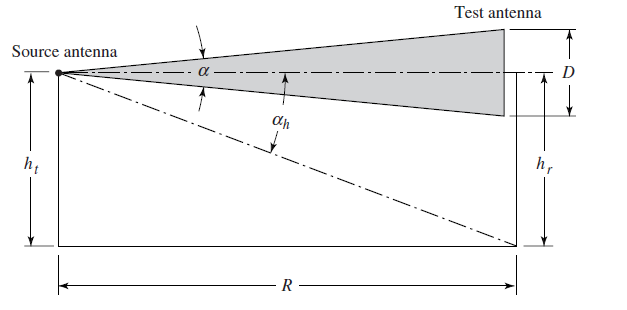
\includegraphics[scale=0.8]{arquitectura instalacion alcance elevado}
    \caption{Esquema de una instalación de alcance elevado extraído de \cite{Balanis_2016}}
    \label{Esquema de una instalación de alcance elevado}
\end{figure}

\newpage

En este tipo de instalaciones las contribuciones del entorno circundante generalmente se reducen o eliminan mediante:

\begin{enumerate}
    \item Una selección cuidadosa de la directividad y de los lóbulos secundarios de la antena de origen.

    \item El despejamiento de obstáculos que impidan tener una la línea de visión clara entre las antenas.

    \item La redirección o absorción de cualquier difracción o reflexión producida durante el proceso de medida.

    \item La utilización de técnicas especiales de procesamiento de señales como el etiquetado de modulación de la señal deseada o el uso de pulsos cortos.
\end{enumerate}

\subsubsection{Alcance inclinado}

Las instalaciones de alcance inclinado sitúan la antena bajo estudio junto con su posicionador en una torre de altura fija que no sea conductora mientras que la antena emisora se sitúa cerca del suelo como se refleja en la siguiente figura:

\begin{figure}[h] 
  \centering
    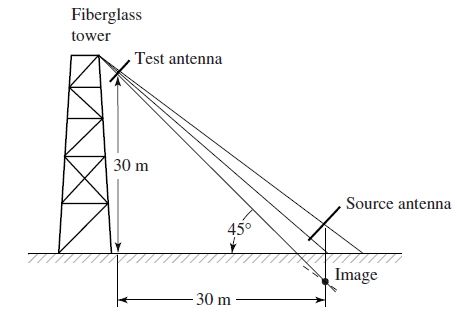
\includegraphics[scale=0.8]{arquitectura instalacion alcance inclinado}
    \caption{Esquema de una instalación de alcance inclinado extraído de \cite{Balanis_2016}}
    \label{Esquema de una instalación de alcance inclinado}
\end{figure}


De este modo, el máximo del patrón de radiación en espacio libre esté orientado hacia el centro de la antena de prueba. Dirigiendo de forma habitual el primer nulo del diagrama de radiación hacia el punto de reflexión estimado que se dará en el suelo para suprimir las señales reflejadas. Este tipo de instalaciones, por regla general, son más compactas que las de tipos elevados en el sentido de que requieren menos espacio para efectuar la medida. 

\newpage

 \subsubsection{Cámaras anecoicas}

Esta instalación proporciona un entorno controlado con una capacidad de simulación de cualquier tipo de clima a la par que proveen seguridad y minimizan radiación electromagnética procedente de fenómenos como la difracción. Las cámaras anecoicas se han desarrollado como una alternativa a las pruebas en exteriores, de forma que las medidas se realizan dentro de una cámara que tiene paredes cubiertas con absorbedores de radio frecuencia.\\

Actualmente, existen dos tipos básicos de diseños de cámaras anecoicas: la cámara rectangular y la cámara cónica. El diseño de cada una se basa en técnicas de óptica geométrica, y ambas intentan reducir o minimizar las reflexiones especulares. La siguiente figura muestra la configuración geométrica de cada una cámara:

\begin{figure}[h] 
  \centering
    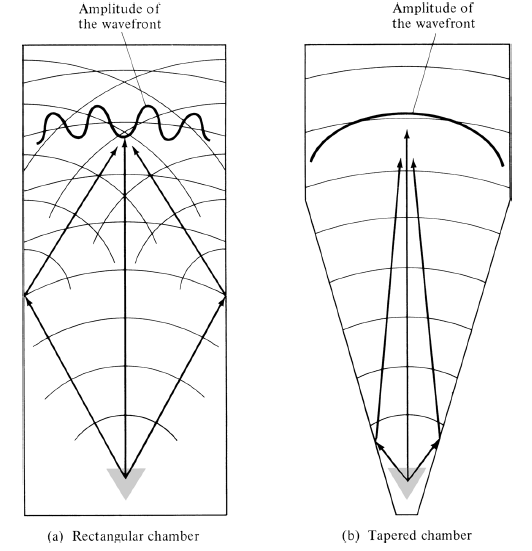
\includegraphics[scale=0.8]{geometría de las cámaras rectangular y cónica}
    \caption{Geometría de las cámaras rectangular y cónica extraido de \cite{Articulo_Kummer}}
    \label{Esquema de una instalación de alcance inclinado}
\end{figure}

La cámara rectangular suele estar diseñada para simular condiciones de espacio libre. El diseño toma en cuenta el patrón y la ubicación de la fuente, la frecuencia de operación, y asume que la antena receptora en el punto de prueba es isotrópica. La energía reflejada se minimiza mediante el uso de absorbentes de RF de alta calidad. A pesar del uso de material absorbente de RF, pueden ocurrir reflexiones especulares significativas, especialmente en ángulos de incidencia grandes.\\

\newpage

Las cámaras anecoicas cónicas tienen la forma de una bocina piramidal. Comienzan con una cámara cónica que conduce a una configuración rectangular en la región de prueba. En el extremo inferior de la banda de frecuencia para la cual la cámara está diseñada, la fuente generalmente se coloca cerca del vértice para que las reflexiones de las paredes laterales, que contribuyen a los campos de iluminación, se minimicen.\\


De entre los dos tipos de instalaciones existentes, este documento únicamente se va a centrar en las instalaciones de alcance en espacio libre. Dado que es el tipo de instalación más común y es sobre el que vamos a trabajar. En el siguiente capítulo encontraremos un análisis más profundo de este tipo de instalaciones, pero antes debemos presentar el método que nos va a permitir tomar medidas de campo lejano en este tipo de instalaciones.

\newpage

\subsection{Método de medida campo cercano a campo lejano}

La toma de medidas se puede reducir notablemente si efectuamos mediciones en campo cercano para luego usar métodos analíticos que nos permitan transformar estos datos calcular así el campo lejano. Este proceso se conoce como campo \textit{campo cercano-campo lejano} (NF/FF abreviado en inglés), y es la técnica empleada como norma general para medir el comportamiento de una antena y en la cual nos basaremos nosotros para efectuar nuestras transformaciones.\\

Este método se usa de forma habitual en cámaras anecoicas para poder realizar las mediciones en un ambiente controlado que proporciona una capacidad ideal para la medición. Sin embargo, como contrapartida, este método requiere de lo siguiente:

\begin{enumerate}
    \item Un sistema complejo que usualmente tiene un precio elevado.
    \item Un proceso de calibración complicado y extenso.
    \item Un software asociado al proceso de medida que debe ser muy sofisticado.
   \item  Una obtención de resultados que no es en tiempo real.
\end{enumerate}

\noindent
Las medidas en campo cercano, usualmente amplitud y fase, se obtienen mediante un escaneo del campo radiado sobre una superficie prefijada que típicamente es un plano, un cilindro o una esfera. La medida de estos datos es traspasada a campo lejano mediante la expresión analítica de la transformada de Fourier. La complejidad de este paso se hace aún mayor en el caso de pasar de una medición sobre una superficie plana a una cilíndrica, o de una cilíndrica a una esférica.\\

La elección del tipo de superficie suele tomarse en función de la antena que deseamos medir, teniendo las siguientes características:

\begin{itemize}
    \item El método de superficie plana es típico en el caso de medir antenas con gran ganancia. Especialmente los \textit{arrays} de fase plana, que requieren de menos carga computacional y no requieren reposicionar la antena.
    \item El método con superficie cilíndrica requiere de una mayor carga computacional comparado con la superficie plana, pero es útil en antenas donde interesa saber su rendimiento en función de la posición de la antena, además de ser el equipo de medida es el más barato de los tres.
    \item El método con superficie esférica es el más costoso en computación y en cuanto al equipo de medida. Da muy buenos resultados si medimos grandes sistemas de antenas. Este método es el que mejor se comporta con equipos de baja ganancia omnidireccionales.
\end{itemize}

\newpage

En un experimento basado en usar una superficie arbitraria, Morse y Feshbach mostraron en \cite{morse&Feshbach1953} que la elección del tipo de superficies es de hecho limitada dado que la derivación del vector de campo lejano a partir del campo cercano depende de que la función del vector de onda sea ortogonal a la superficie empleada. En base a esto, los seis sistemas de coordenadas válidos son el plano, el circular, el cilíndrico, el esférico, el cilíndrico elíptico, el cilíndrico parabólico y el cónico. Los tres primeros sistemas de coordenadas están orientados a la adquisición de datos, mientras que los tres últimos requieren pasar cilindros elípticos, cilindros parabólicos o esferas a coordenadas cónicas. Es por esto que las tres técnicas de campo cercano a campo lejano que se han desarrollado están basadas en ondas planas, cilíndricas o esféricas.\\

\begin{figure}[h] 
  \centering
    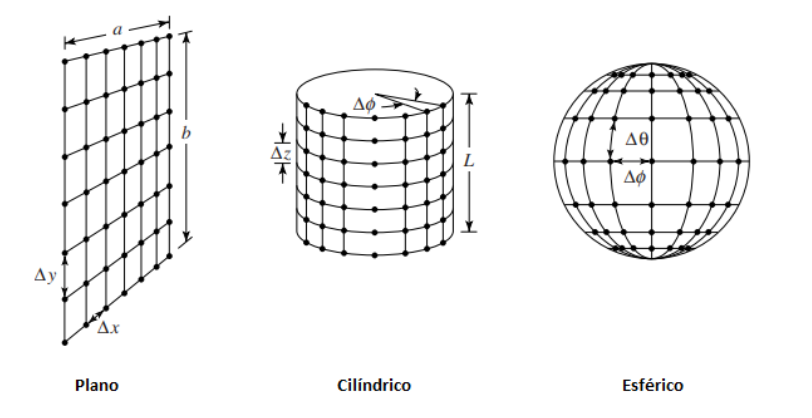
\includegraphics[scale=0.5]{sistemas de coordenadas}
    \caption{Sistemas de coordenadas empleados en el método de campo cercano a campo lejano}
    \label{Sistemas de coordenadas empleados en el método de campo cercano a campo lejano}
\end{figure}

La adquisición de datos de un campo cercano planar generalmente se realiza a través de una malla rectangular como la de la figura \ref{Sistemas de coordenadas empleados en el método de campo cercano a campo lejano}. En esta malla, el máximo espaciado de las muestras sigue la relación $\Delta x = \Delta y = \lambda/2$ . También es posible adquirir esta medida empleando una malla plana polar o una malla bipolar. En caso de usar una superficie plana, la antena bajo medida deberá estar estacionada mientras que la antena transmisora (usualmente una antena tipo bocina) se podrá mover a través de cualquier punto de la malla. Es fundamental tener en cuenta la directividad y polarización de nuestra antena transmisora, ya que esto debe tenerse en cuenta cuando empleemos técnicas de compensación.\\ 

Estos métodos de compensación de la antena transmisora emplean el teorema de reciprocidad de Lorentz para emparejar los campos lejanos de la antena a estudiar con los de la antena transmisora. La principal ventaja de la transformación de campo cercano a lejano planar sobre el cilíndrico o esférico es su simplicidad matemática.  Además, la transformación planar se puede sustituir aplicando computacionalmente la transformada de Fourier. Si asumimos que el número puntos es $2^n$, siendo $n$ positivo y entero, la transformada del campo completo planar puede obtenerse computacionalmente en un tiempo proporcional a: 

\begin{equation}
    t = (ka)2\log_2(ka)
    \label{proporcion temporal cálculo de fourier}
\end{equation}

\noindent
donde $a$ es el radio del círculo más pequeño descrito por la antena bajo estudio. La transformada planar está muy bien descrita para la medida de antenas con lóbulos traseros pequeños. Esto hace referencia a antenas de bocina, reflectores o arrays planos. 

\newpage

La principal ventaja de obtener los datos en campo cercano y extrapolar a campo lejano es que el patrón obtenido en campo lejano está limitado en pasos angulares. Esto implica que, si el escaneo de la superficie se hiciese con infinitos puntos, podríamos obtener computacionalmente un hemisferio del campo lejano sin ningún tipo de error. La medida por completo del campo lejano sobre superficies cilíndricas incluye además la información necesaria para, de forma computacional, obtener un patrón completo en azimut para todos los ángulos de elevación. Aunque esto no incluye ni a las regiones cónicas ni las tapas del propio cilindro.\\

En cuanto al uso de superficies esféricas, la información obtenida mediante el escaneo del campo lejano hace posible la predicción completa del patrón de radiación en campo lejano. Es decir, cualquier patrón de campo lejano puede ser computacionalmente obtenido a partir de la medida en campo cercado con un escaneo esférico. Otra ventaja añadida es que el escaneo esférico corrige típicamente la posición y orientación de la antena a medir y varía su orientación angular hacia la antena transmisora. Debido a que la antena transmisora siempre apunta directamente a la antena transmisora, la corrección de la antena transmisora puede ser pasar por alto si empleamos un escaneo con un campo lo suficientemente grande.\\

Pese a todo lo anterior, la principal desventaja del escaneo esférico radica en la transformada matemática. Una porción significativa de la transformada no puede realizarse a través de la FTT para lo cual empleamos integración numérica, operaciones con matrices y soluciones simultaneas de ecuaciones. Esto incrementa mucho la carga computacional y dificulta la transformación considerablemente con respecto al caso plano o cilíndrico.\\

\newpage

\section{Sobre las herramientas utilizadas}

Antes de entrar en profundidad en el contenido principal del documento, debemos comentar las herramientas principales que hemos utilizado durante el desarrollo del mismo.

\begin{itemize}
    \item \textbf{COMSOL}: Nos hemos apoyado en COMSOL como herramienta de simulación para poder construir y estudiar modelos de antenas. Gracias a este programa hemos podido generar conjuntos de datos que nos han permitido poner en práctica nuestras transformaciones y, de forma adicional, verificar que los resultados obtenidos coincidían con los proporcionados por la simulación.

    \item \textbf{Python}: Hemos utilizado Python como lenguaje de programación principal por sus muchas ventajas frente a otras opciones. Algunas de estas son disponer de librerías que nos faciliten mucho el trabajo a la hora de tratar con herramientas tales como la transformada de fourier, su flexibilidad a la hora de ejecutar el programa en cualquier sistema operativo, su comunidad activa y la velocidad en el desarrollo de los programas.

    \item \textbf{Wolfram Matematica}: Durante el desarrollo de las transformaciones necesitábamos disponer de otro conjunto de resultados que nos permitiese verificar los resultados de Python. Este hecho motivó el uso de Wolfram Matematica para desarrollar las transformaciones en este programa de forma paralela y así poder tener datos con los que comparar las transformaciones. La elecicón de este programa por encima de otros se debe a que ya dispone de muchas herramientas matemáticas necesarias para hacer la transformación como son las ecuaciones de Legendre o las de Hankel y su facilidad a la hora de programar ecuaciones complejas.
\end{itemize}